\documentclass[a4paper]{extarticle}
\usepackage{ctex}
\usepackage{titlesec}
\usepackage{lipsum}
\usepackage{geometry}
\usepackage{amsmath}
\usepackage{biblatex}
\usepackage{booktabs}
\usepackage{caption}
\usepackage{graphicx}
\usepackage{float}
\setCJKmainfont{STSong}[AutoFakeBold,AutoFakeSlant]
\setCJKsansfont{Microsoft YaHei}
\setCJKmonofont{KaiTi}
\setmainfont{Times New Roman}
\setsansfont{Times New Roman}
\setmonofont{Times New Roman}
\linespread{1.5}
\setlength{\parindent}{0pt}
\titleformat{\section}{\bfseries\fontsize{14pt}{\baselineskip}\selectfont}{\thesection}{0.5em}{}
\titleformat{\subsection}{\bfseries\fontsize{10.5pt}{\baselineskip}\selectfont}{\thesubsection}{0.5em}{}
\titleformat{\subsubsection}{\fontsize{10.5pt}{\baselineskip}\selectfont}{\thesubsubsection}{0.5em}{}
\geometry{left=2.5cm,right=2.5cm,top=2.5cm,bottom=2.5cm}
\everymath{\displaystyle}

\begin{document}
    \begin{center}
        \textbf{\fontsize{22pt}{\baselineskip} \selectfont 单摆法测重力加速度}\\
        \vspace{2em}
        \texttt{\fontsize{14pt}{\baselineskip} \selectfont 作者:刘子墨,学号:PB23000233}\\
    \end{center}
    \vspace{2em}
    \textsf{\fontsize{9pt}{\baselineskip} \selectfont 摘要:}
    \texttt{\fontsize{9pt}{\baselineskip} \selectfont 本实验探究采用单摆法对合肥的重力加速度进行了测量。在满足1\%测量精度的要求下,设计并优化了实验方案。通过对周期的累积放大,提高了测量精度。最终测得合肥的重力加速度值为9.796 m/s$^2$,其标准不确定度为0.036 m/s$^2$满足实验的测量精度要求。此外,还通过调整单摆的摆长,测量了周期$T$与摆长$l$的变化关系,并对$l$与$T^2$的关系进行了线性拟合,从而得到了重力加速度的值为9.822 m/s$^2$。最后,通过视频追踪,我们分析了大摆角下单摆的运动轨迹,进一步研究了摆角和空气阻力对单摆周期的影响。}\\
    \textsf{\fontsize{9pt}{\baselineskip} \selectfont 关键词:}
    \texttt{\fontsize{9pt}{\baselineskip} \selectfont 单摆、重力加速度、累积放大法、视频追踪、不确定度分析}
    \section{引言}
    \hspace{2em}
    单摆实验是一个经典实验,许多著名的物理学家如伽利略、牛顿、惠更斯等都对单摆实验进行过细致的研究。伽利略发现了摆的等时性原理,指出摆的周期与摆长的平方根成正比,而与摆的质量和材料无关,为后来摆钟的设计与制造奠定了基础。1673 年荷兰科学家惠更斯制造的惠更斯摆钟就运用了摆的等时性原理。摆的等时性原理应用于时钟上,作为稳定的“定时器”,使机械钟能够指示出“秒”,从而将计时精度提高了近 100 倍。
    \par\hspace{2em}
    理想的单摆,是一根没有质量、没有弹性的线,系住一个没有体积的质点,在真空中由于重力作用而在与地面垂直的平面内做摆角趋于零的自由振动。这种理想的单摆,实际上是不存在的。在实际的单摆实验中,悬线是一根有质量(弹性很小)的线,摆球是有质量有体积的刚性小球,摆角不为零,摆球的运动还受到空气的影响。
    \par\hspace{2em}
    单摆的周期公式为:
    \begin{equation*}
        T=2\pi\sqrt{\frac{l}{g}\left[1+\frac{d^2}{20l^2}-\frac{m_0}{12m}\left(1+\frac{d}{2l}+\frac{m_0}{m}\right)+\frac{\rho_0}{2\rho}+\frac{\theta^2}{16}\right]}
    \end{equation*}
    其中,$T$为周期,$l$为摆长,$g$为重力加速度,$d$为线的直径,$m_0$为线的质量,$m$为摆球的质量,$\rho_0$为空气的密度,$\rho$为摆球的密度,$\theta$为摆角。一般情况下,摆球几何形状、摆线
    的质量、空气浮力、摆角($\theta<5^{\circ}$)对$T$的修正都小于$10^{-3}$。本实验中,精度要求在$1\%$以内,因此可以忽略这些修正项。此时,周期公式可以近似为:
    \begin{equation*}
        T=2\pi\sqrt{\frac{l}{g}}
    \end{equation*}
    则可以通过测量周期$T$和摆长$l$,计算出重力加速度$g$。
    \section{实验内容与设计}
    \subsection{实验仪器}
    \hspace{2em}
    钢卷尺、电子秒表、单摆(带标尺、平面镜;摆线长度可调,其可调的上限约为 100 cm)。
    \subsection{实验方案设计}
    \hspace{2em}
    由单摆周期公式得,重力加速度的测量公式为:
    \begin{equation*}
        g=\frac{4\pi^2l}{T^2}
    \end{equation*}
    则重力加速度的标准合成不确定度公式为:
    \begin{equation*}
        \mu_g=\sqrt{\left(\frac{\partial g}{\partial l}\right)^2\mu_L^2+\left(\frac{\partial g}{\partial T}\right)^2\mu_T^2}=g\sqrt{\left(\frac{\mu_L}{L}\right)^2+\left(\frac{2\mu_T}{T}\right)^2}
    \end{equation*}
    \par\hspace{2em}
    通过单摆周期公式,可以得到摆长为 70 cm 时,按合肥重力加速度为 9.795 m/s$^2$计算,单摆的周期约为 1.68 s。如果测量单个周期的相对不确定度为:$\frac{0.2}{1.68}$ = 12\%,远大于 1\%的精度要求。故必须使用累积放大法测量多个周期的累积时间才能满足测量精度的要求。
    \par\hspace{2em}
    设测量n个周期,累积时间为$T_n$,则重力加速度的不确定度合成公式为:
    \begin{equation*}
        \mu_g=g\sqrt{\left(\frac{\mu_L}{L}\right)^2+\left(\frac{2\mu_T}{nT}\right)^2}<1\%
    \end{equation*}
    可得$n>26$,即测量26个周期的累积时间,可以满足 1\% 的测量精度要求。所以在实验中选择测量30个周期。
    \subsection{实验内容}
    \subsubsection{基础内容}
    \hspace{2em}
    根据所设计的方案测量单摆的摆长和周期,要求摆长和周期分别重复测量6次。计算当地的重力加速度及其标准不确定度。
    \subsubsection{提升内容}
    \hspace{2em}
    调节单摆的摆长,测量摆长$l$与周期$T$之间的关系。要求测量6个不同的摆长。做出$l$与$T^2$之间的关系图,并用最小二乘法拟合斜率,求出重力加速度。
    \subsubsection{进阶内容}
    \hspace{2em}
    利用智能手机录制单摆视频。用视频追踪技术(Tracker)获取单摆的运动轨迹,研究大摆角($>5^{\circ}$)条件下单摆的运动规律。对运动轨迹数据进行拟合分析。
    \section{实验结果和讨论}
    \subsection{摆长和周期求重力加速度}
    \hspace{2em}
    通过测量单摆的摆长和周期,得到了如下数据:
    \begin{table}[H]
        \centering
        \caption{单摆摆长和周期的测量数据}
        \begin{tabular}{cccc}
            \toprule
            组别&摆长$l$/cm&30周期$30T$/s&周期$T$/s\\
            \midrule
            1&62.80&47.75&1.5916\\
            2&62.80&47.72&1.5906\\
            3&62.70&47.76&1.5920\\
            4&62.90&47.56&1.5853\\
            5&62.90&47.79&1.5930\\
            6&62.80&47.82&1.5940\\
            \midrule
            平均值&62.817&47.733&1.5911\\
            \bottomrule
        \end{tabular}
    \end{table}
    \par\hspace{2em}
    将测得周期和摆长的估计值带入单摆周期公式,得到重力加速度测量值为:
    \begin{equation*}
        g=\frac{4\pi^2l}{T^2}=\frac{4\pi^2\times0.62817}{1.5911^2}=9.7958\,\text{m/s}^2
    \end{equation*}
    \subsubsection{摆长的不确定度评定}
    \hspace{2em}
    实验使用钢卷尺测量摆长。摆长的测量模型为:
    \begin{equation*}
        L=\overline{L}+L_0+L_1
    \end{equation*}
    其中$\overline{L}$为钢卷尺直接读出的摆长,$L_0$为钢卷尺的仪器误差对测量的影响,$L_1$为使用卷尺测量摆长时难以完全对齐对测量结果的影响,作为保守估计,一般可取最大不确定度$\Delta_B\approx$ 0.2 cm。考虑到测量精度要求,测量模型中忽略了其他因素的影响。
    \par\hspace{2em}
    钢卷尺直接读出的摆长$\overline{L}$为A类,其不确定度$\mu_{\overline{L}}$为:
    \begin{equation*}
        \mu_{\overline{L}}=\sqrt{\frac{\sum\limits_{i=1}^{n}(L_i-\overline{L})^2}{n(n-1)}}=3.1\times10^{-4}\,\text{m}
    \end{equation*}
    钢卷尺的仪器误差$L_0$为B类正态分布,实验中用 2 m 量程钢卷尺的最大允差为 0.0012
    m,其不确定度$\mu_{L_0}$为:
    \begin{equation*}
        \mu_{L_0}=\frac{\Delta_\text{尺}}{3}=4\times10^{-4}\,\text{m}
    \end{equation*}
    \hspace{2em}
    使用卷尺测量摆长时难以完全对齐对测量结果的影响$L_1$呈B类正态分布,取最大不确定度$\Delta_B\approx$ 0.2 cm,则其不确定度为:
    \begin{equation*}
        \mu_{L_1}=\frac{\Delta_B}{3}=6.67\times10^{-4}\,\text{m}
    \end{equation*}
    \hspace{2em}
    所以摆长的不确定度为:
    \begin{equation*}
        \mu_L=\sqrt{\mu_{\overline{L}}^2+\mu_{L_0}^2+\mu_{L_1}^2}=8.3\times10^{-4}\,\text{m}
    \end{equation*}
    \subsubsection{周期的不确定度评定}
    \hspace{2em}
    实验使用秒表每次测量 30 个周期的时长,摆动周期$T$的测量模型为;
    \begin{equation*}
        T=(\overline{T}+T_0+T_1)/30
    \end{equation*}
    其中$\overline{T}$为秒表直接读出的周期,$T_0$为秒表的仪器误差对测量的影响,$T_1$为使用秒表计时时人的反应时间对测量的影响。根据统计分析,实验人员开启或停止秒表的反应时间为 0.1 s 左右,所以实验人员测量时间的精度近似为$\Delta_\text{人}\approx$0.2 s。考虑到测量精度要求,测量模型中忽略了其他因素的影响。
    \par\hspace{2em}
    秒表直接读出的周期$\overline{T}$为A类,其不确定度$\mu_{\overline{T}}$为:
    \begin{equation*}
        \mu_{\overline{T}}=\sqrt{\frac{\sum\limits_{i=1}^{n}(T_i-\overline{T})^2}{n(n-1)}}=0.033\,\text{s}
    \end{equation*}
    \par\hspace{2em}
    秒表的仪器误差$T_0$为B类正态分布,实验中使用的电子秒表的最大允差为 0.05 s,其不确定度$\mu_{T_0}$为:
    \begin{equation*}
        \mu_{T_0}=\frac{\Delta_\text{表}}{3}=0.017\,\text{s}
    \end{equation*}
    \par\hspace{2em}
    使用秒表计时时人的反应时间$T_1$呈B类正态分布。根据统计分析,实验人员开启或停止秒表的反应时间为 0.1 s 左右,实验人员测量时间的精度近似为$\Delta_\text{人}\approx$0.2 s。则其不确定度为:
    \begin{equation*}
        \mu_{T_1}=\frac{\Delta_\text{人}}{3}=0.067\,\text{s}
    \end{equation*}
    \par\hspace{2em}
    所以周期的不确定度为:
    \begin{equation*}
        \mu_T=\frac{1}{30}\sqrt{\mu_{\overline{T}}^2+\mu_{T_0}^2+\mu_{T_1}^2}=2.7\times10^{-3}\,\text{s}
    \end{equation*}
    \subsubsection{重力加速度的标准不确定度评定}
    \hspace{2em}
    重力加速度的测量模型为:
    \begin{equation*}
        g=\frac{4\pi^2l}{T^2}
    \end{equation*}
    \par\hspace{2em}
    重力加速度的标准不确定度为:
    \begin{equation*}
        \mu_g=g\sqrt{\left(\frac{\mu_L}{L}\right)^2+\left(\frac{2\mu_T}{T}\right)^2}=0.036\,\text{m/s}^2
    \end{equation*}
    \par\hspace{2em}
    即重力加速度的测量结果可表示为:$g=(9.796\pm0.036)\,\text{m/s}^2$。
    \subsection{改变摆长利用摆长和周期拟合求重力加速度}
    \hspace{2em}
    通过调整单摆的摆长,测量了周期$T$与摆长$l$的变化关系,得到了如下数据:
    \begin{table}[H]
        \centering
        \caption{单摆摆长和周期的测量数据}
        \begin{tabular}{ccccc}
            \toprule
            组别&摆长$l$/cm&30周期$30T$/s&周期$T$/s&$T^2$\\
            \midrule
            1&55.10&44.71&1.4903&2.2211\\
            2&62.80&47.75&1.5917&2.5334\\
            3&69.00&50.00&1.6667&2.7778\\
            4&77.80&53.18&1.7727&3.1424\\
            5&86.20&55.94&1.8647&3.4870\\
            6&94.10&58.36&1.9453&3.7843\\
            \bottomrule
        \end{tabular}
    \end{table}
    \par\hspace{2em}
    通过线性拟合,得到了摆长$l$与周期$T^2$的关系图:
    \begin{figure}[H]
        \centering
        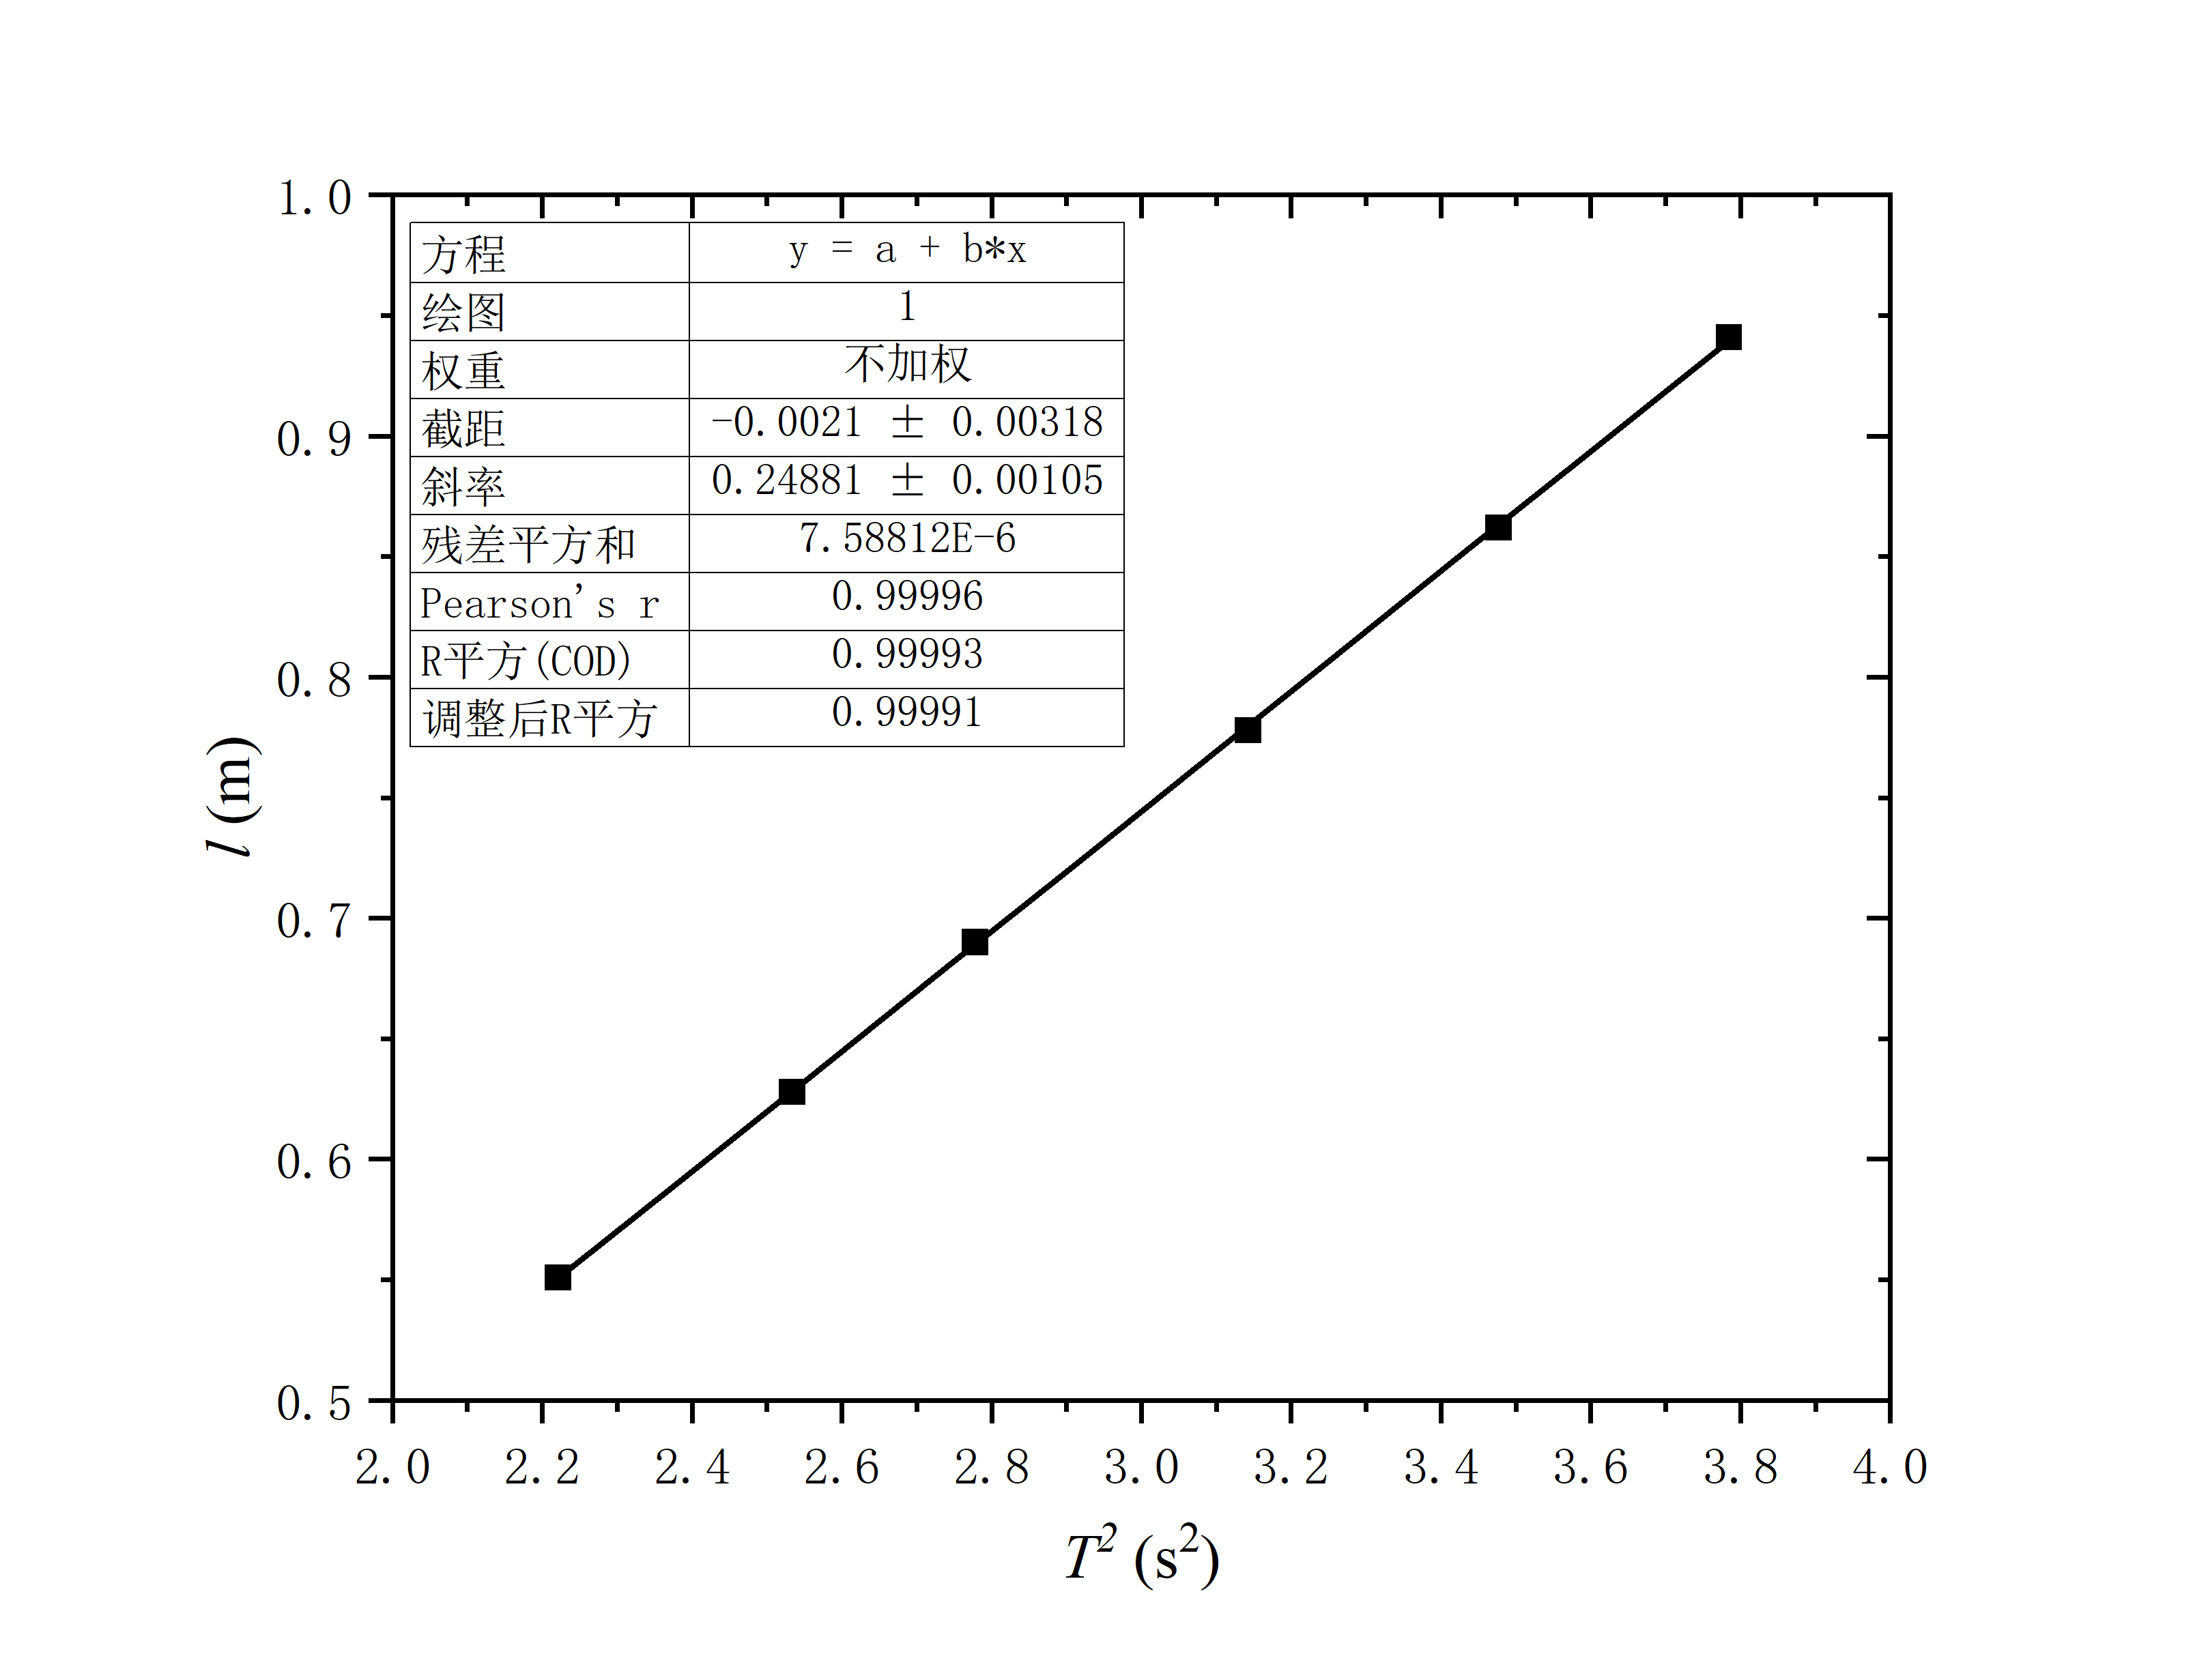
\includegraphics[width=\linewidth]{1.png}
        \caption{摆长$l$与周期$T^2$的关系图}
    \end{figure}
    \par\hspace{2em}
    通过最小二乘法拟合斜率,得到了斜率$k$的数值为0.2488,则重力加速度的值为:
    \begin{equation*}
        g=4\pi^2k=9.822\,\text{m/s}^2
    \end{equation*}
    \par\hspace{2em}
    其标准不确定度为:
    \begin{equation*}
        \mu_g=4\pi^2\mu_k=0.041\,\text{m/s}^2
    \end{equation*}
    \subsection{利用视频追踪技术研究大摆角下单摆的运动规律}
    \hspace{2em}
    将手机固定在实验室提供的手机支架上,录制了一段帧率为60FPS的大角度单摆(摆角约为 12°)视频,并使用tracker软件进行自动追踪分析。Tracker 从该视频中获取有效数据点2009个,并导入origin进行正弦函数拟合。结果如下:
    \begin{figure}[H]
        \centering
        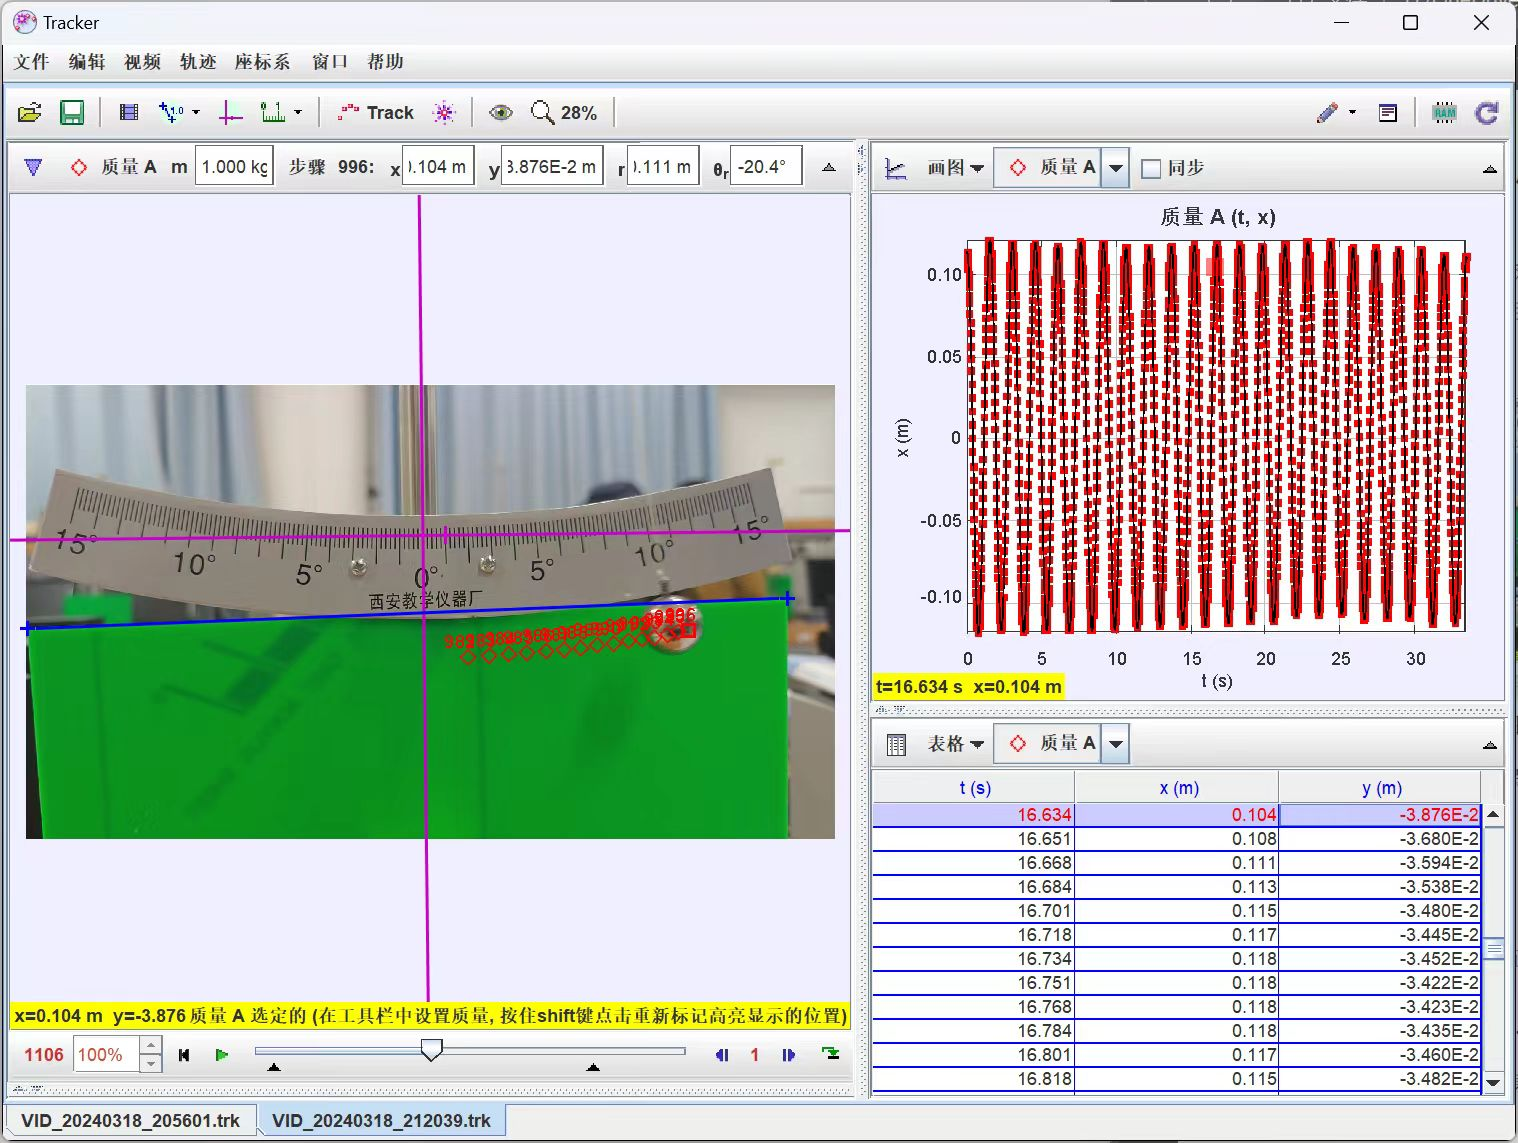
\includegraphics[width=\linewidth]{2.jpg}
        \caption{使用tracker软件追踪的单摆运动轨迹}
    \end{figure}
    \begin{figure}[H]
        \centering
        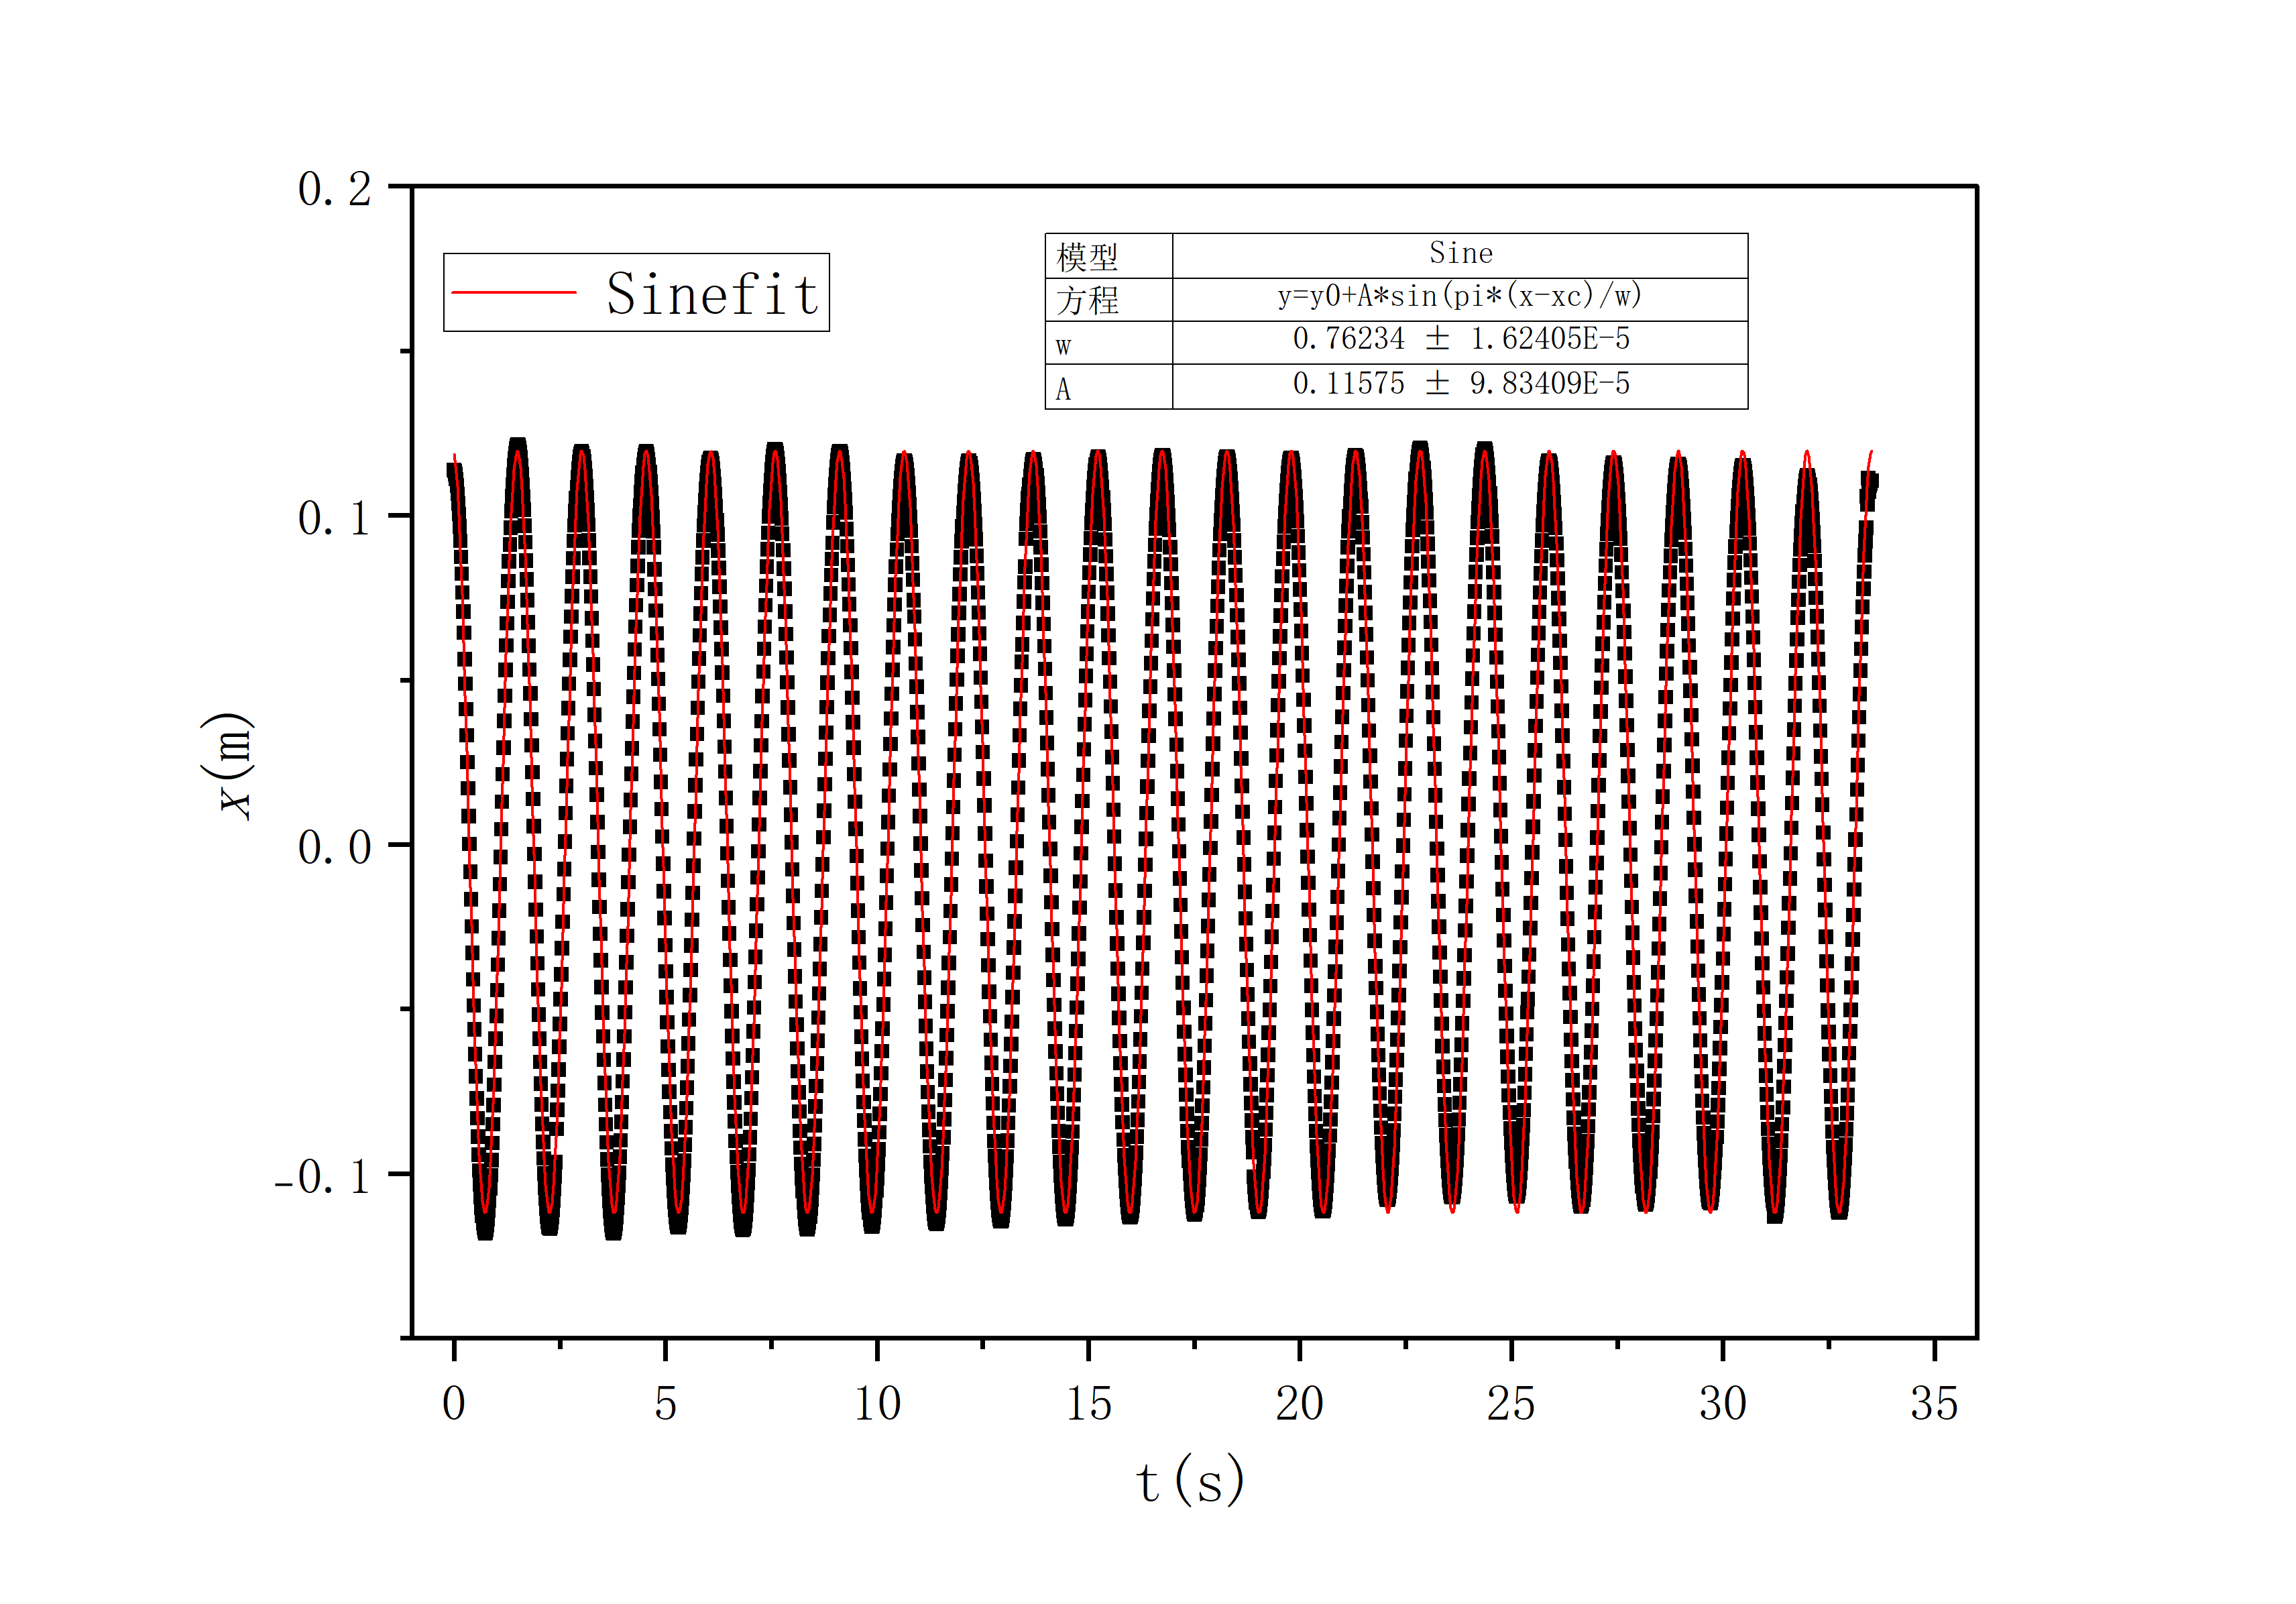
\includegraphics[width=\linewidth]{3.png}
        \caption{单摆水平方向运动轨迹的正弦函数拟合结果}
    \end{figure}
    \par\hspace{2em}
    拟合结果给出单摆的摆动周期$T=$1.5246 s。利用卷尺测得的单摆摆长$l=$0.574 m,带入未修正的单摆测重力加速度的公式可得:
    \begin{equation*}
        g=\frac{4\pi^2l}{T^2}=9.749\,\text{m/s}^2
    \end{equation*}
    \par\hspace{2em}
    若考虑大摆角下的修正,则重力加速度为::
    \begin{equation*}
        g=\frac{4\pi^2l}{T^2}\left(1+\frac{1}{4}\sin^2\left(\frac{\theta}{2}\right)\right)=9.802\,\text{m/s}^2
    \end{equation*}
    \par\hspace{2em}
    可以看到修正后的结果与合肥的重力加速度参考值9.795 m/s$^2$更加接近。
    \section{结论}
    \hspace{2em}
    本文基于单摆实验装置利用三种不同的方案测量了合肥的重力加速度,测量结果分别为:9.796 m/s$^2$、9.822 m/s$^2$和9.802 m/s$^2$,与参值9.795的偏差均小于1\%。在 10°的大摆角情况下研究了摆角和空气阻力对单摆周期的影响,结果表明考虑摆角修正后测得的重力加速度更接近参考值,修正对测量结果的影响约为 \%;而阻力对单摆周期的修正约为,远小于 1\%。因此,小角度摆动条件下在实验测量精度的范围内完全可以忽略相关因素对测量结果的影响。
    \section*{参考文献}
    [1]. 单摆法测重力加速度. 实验讲义. 2024
    \par
    [2]. 舒幼生. 力学[M]. 北京:北京大学,2005.
    \par
    [3]. 邵云. 单摆周期的系统误差分析[J]. 大学物理, 2022, 41(01): 32-38.
    \newpage
    \section*{附录}
    \subsection*{老师签字的实验数据}
    \begin{figure}[H]
        \centering
        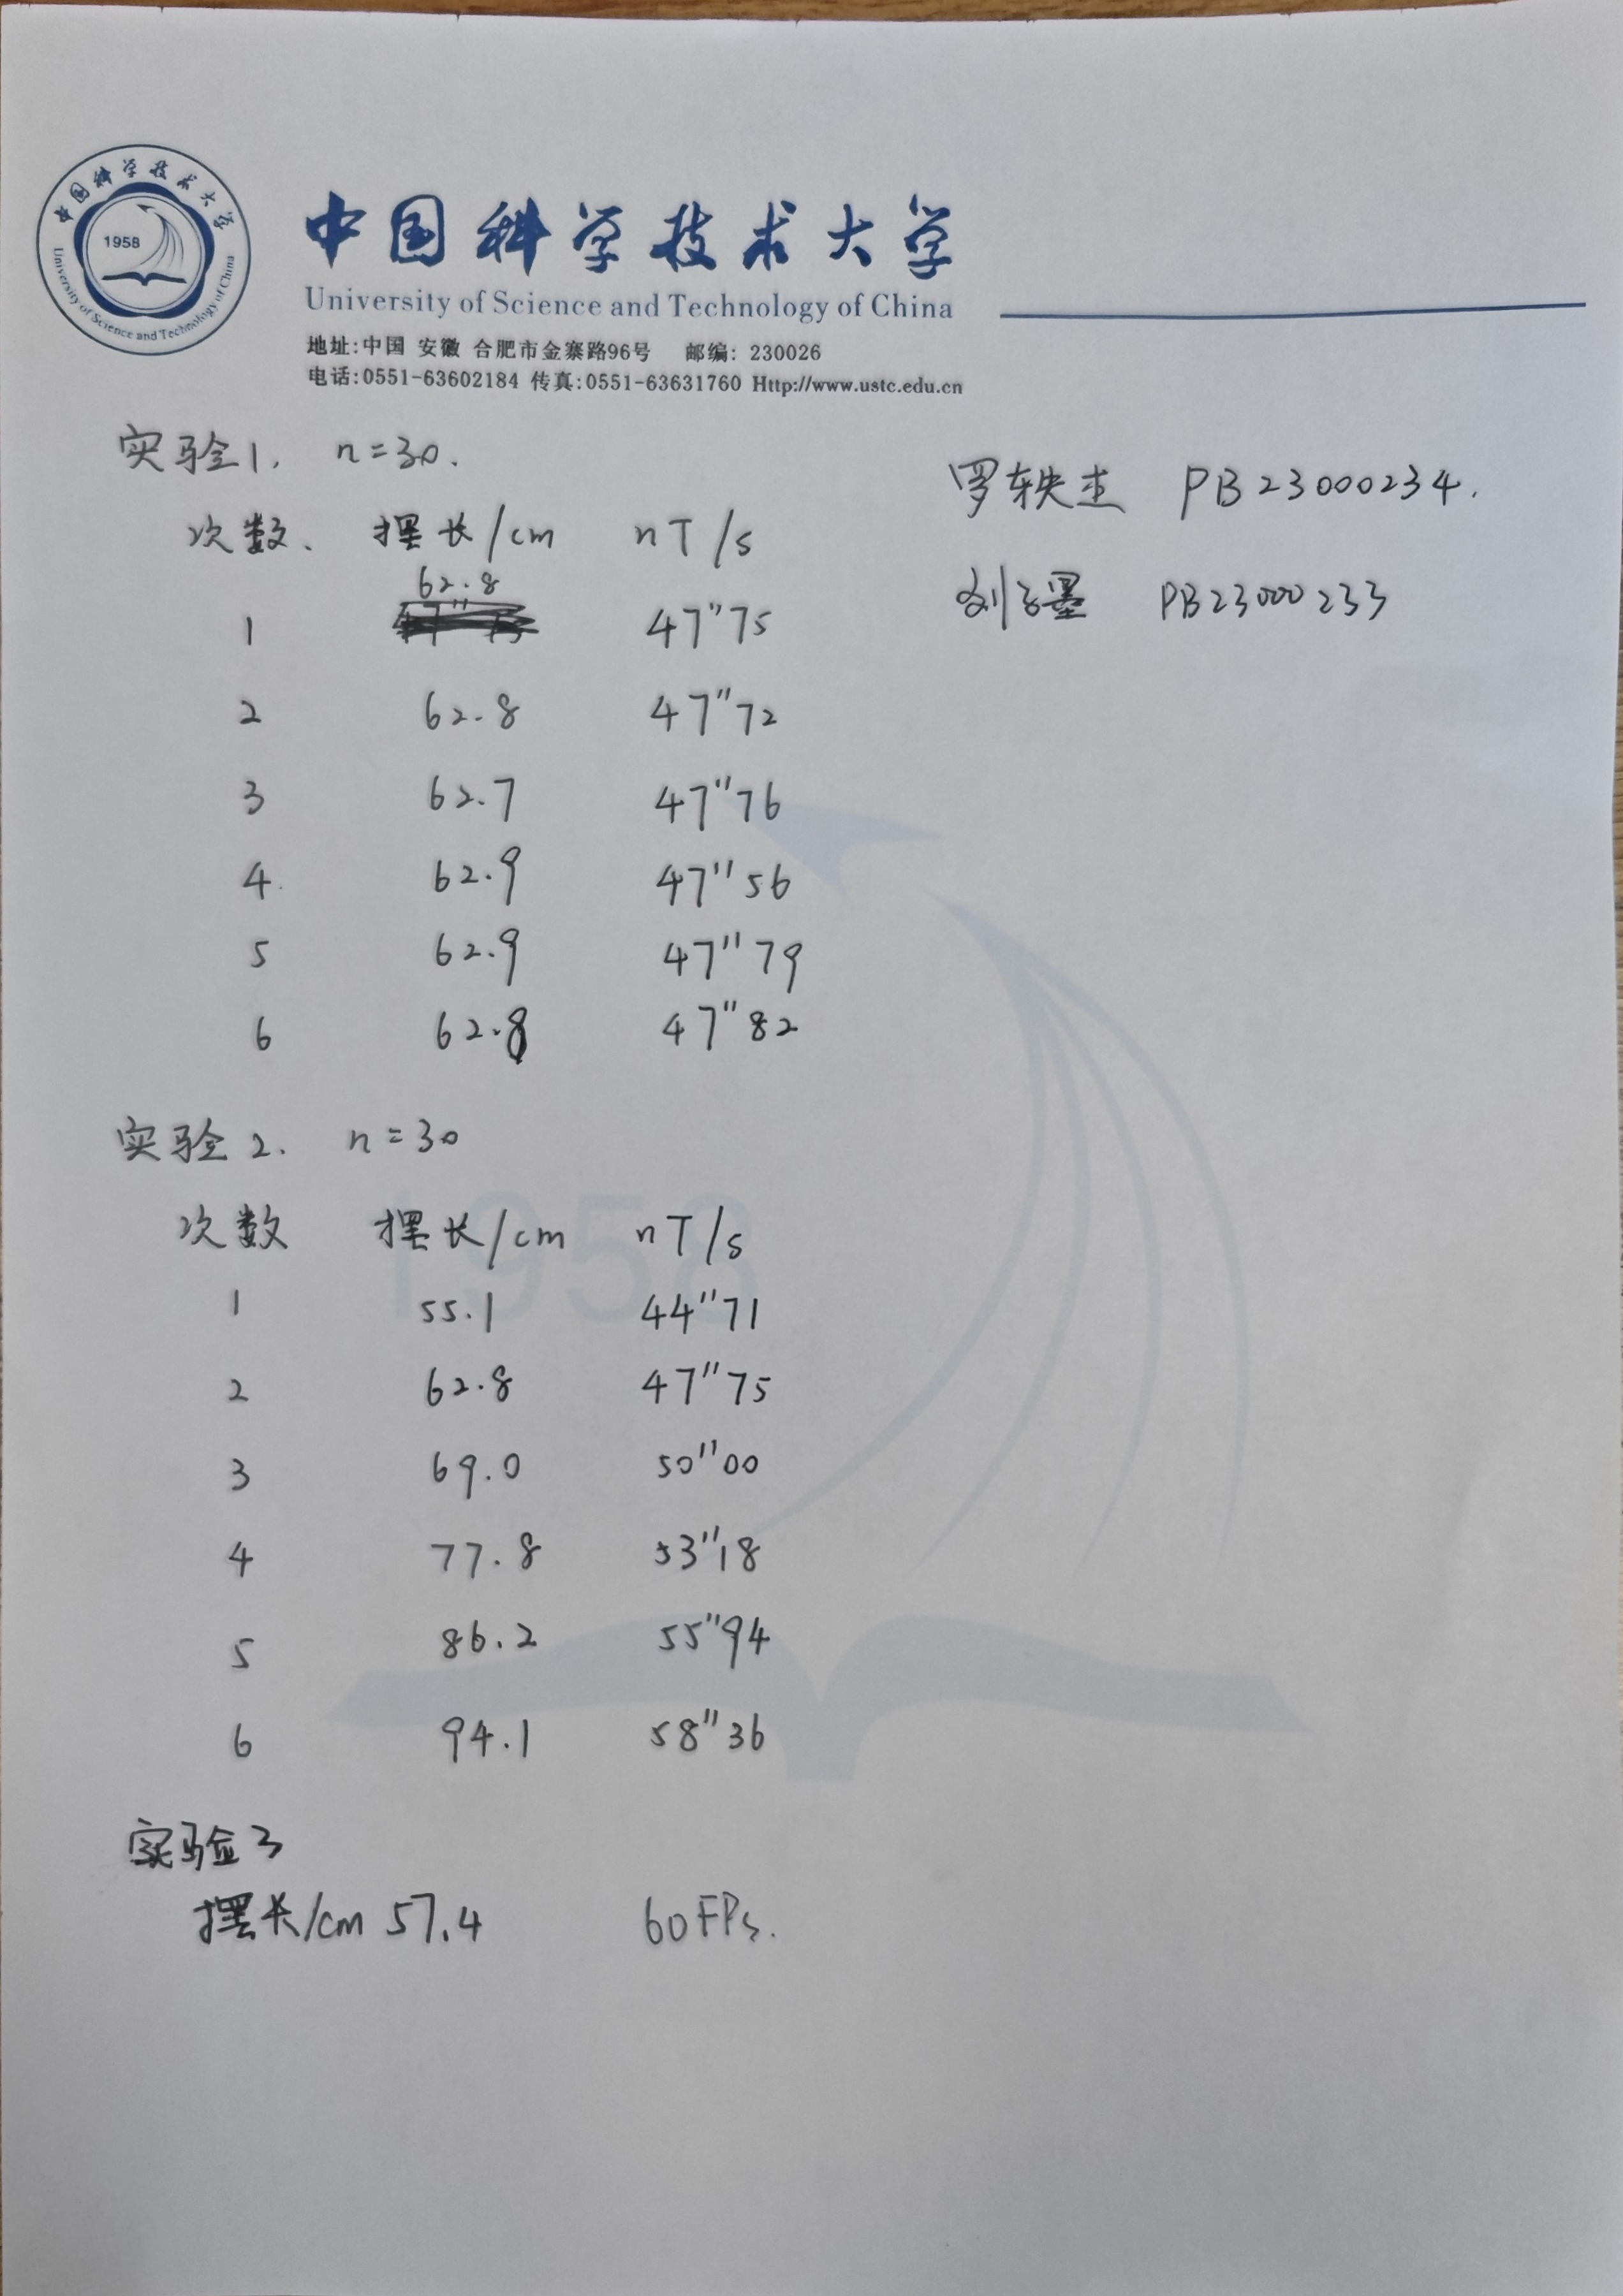
\includegraphics[width=\linewidth]{4.jpg}
    \end{figure}
\end{document}
